\documentclass[twocolumn,11pt]{article}
\setlength{\textheight}{9truein}
\setlength{\topmargin}{-0.9truein}
\setlength{\parindent}{0pt}
\setlength{\parskip}{10pt}
\setlength{\columnsep}{.4in}

\usepackage{amsmath,amsfonts,amssymb,amsthm,bm,caption,calc,ifthen,graphicx,url,hyperref}

\begin{document}
\pagestyle{plain}
\onecolumn
PHYS689 
\newline Homework 3
\newline Will Wainwright
\newline Repository: \href{https://github.com/wjwainwright/PHYS689}{https://github.com/wjwainwright/PHYS689}

\section*{Discussion}
For this assignment I determined the acceleration due to gravity in two different ways. The first way I did this was by averaging the three times recorded for each pendulum length and calculating g for that pendulum length. I then averaged the g determined across each trial and recorded that as the overall g value. For the uncertainty I propagated the error through the formula $dG =  \sqrt{(\frac{4\pi^2dL}{{\bar T}^2})^2 + (\frac{8\pi^2LdT}{\bar T^3})^2}$. From this method I got an answer of $g=(9.8139 \pm 0.0897) m/s$. 

I then constructed a plot of the period squared as a function of length. The slope of this plot should therefore be $m=\frac{T^2}{L} = \frac{4\pi^2}{g}$. I fit the data points using Numpy's polyfit method, which yielded a value of $m=4.00479 s^2/m$ and therefore $g=(9.8578 \pm 0.009) m/s$. The uncertainty for the graphical method is far too low in reality. The $0.009m/s$ comes from the uncertainty in the fit according to Numpy's polyfit. Polyfit does not take into account uncertainties in the data points, namely dT and dL, and so therefore the actual uncertainty should be closer to what was determined through propagation.

\begin{figure}[!h]
	\centering
	\noindent
	\makebox[\textwidth]{
      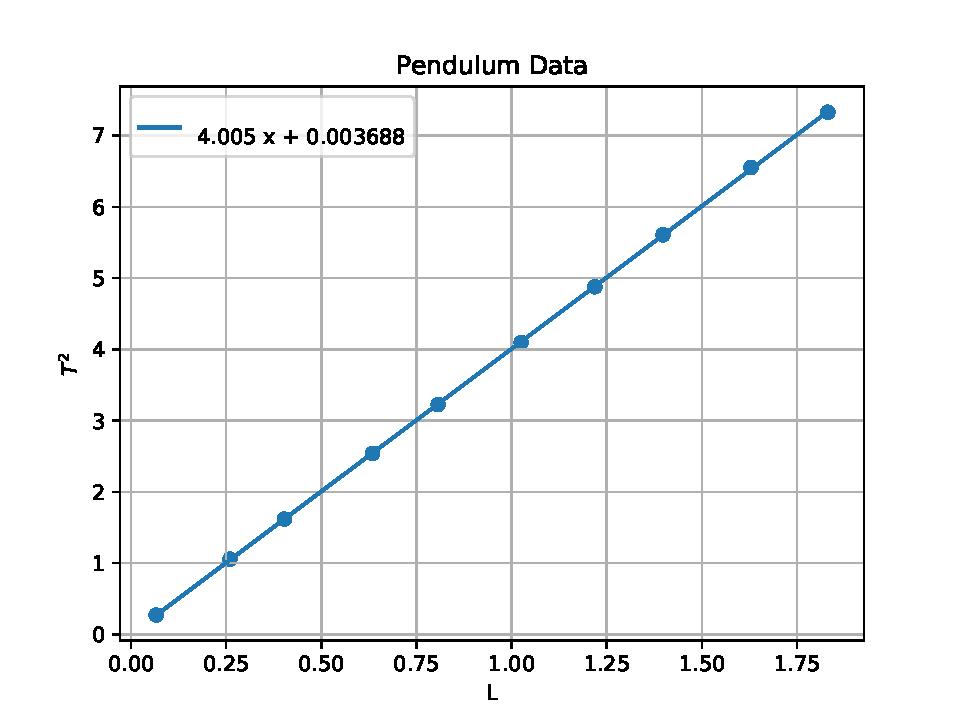
\includegraphics[width=5in]{plot.pdf}}
      \caption{}
\end{figure}

As for a comparison of the different methods, the stepwise method came a lot closer to the actual answer, but the linear fit is closer to what one would usually do with a data set like this and a model equation. Even though the accepted value is outside of the uncertainty range on the plot's fit, if you take into account uncertainty in L and T and assume an uncertainty closer to that of the propagation method then the fit agrees with the accepted value. Even if the fit were to not agree with the accepted value, I would assume some type of systematic error present in the process of data collection. The point of taking multiple sets of data is to reduce any random noise that may be present, but a systematic error could still skew a data set such as this one. The only aspect of my handling of uncertainty that should help with systematic error is the timing of 10 periods versus one, and then times being divided by 10. This should reduce any systematic errors in time by a factor of 10, but won't affect any systematic errors in length. 

Assuming a null hypothesis that the model equation given is correct, I propose an alternative hypothesis that g should really be related to a linear slope $m=\frac{T^2}{L}=\frac{2e}{g}$. To test the data against this hypothesis I took the slope $m=4.00479 s^2/m$ and then calculated a value of $g=(1.3575 \pm 0.009) m/s$. When approaching the question of whether to accept or reject the null hypothesis, I agree with the sentiment that extraordinary claims require extraordinary evidence. Not only do I lack confidence in the quality of the uncertainty interval, but I lack any form of derivation or theory to back up the model which I am saying fits my data. For these reasons and more, I'm going to accept the null hypothesis and assume that physics is correct on this one.



\end{document}